\section{Clustering}
\label{sect:clustering}

In the first step of the pipeline, we cluster the input graph. We take the static, simple input graph and compute clusters of vertices and their similarities. This yields a complete vertex- and edge-weighted graph that we call the \emph{cluster graph}.

\begin{figure}[H]
	\centering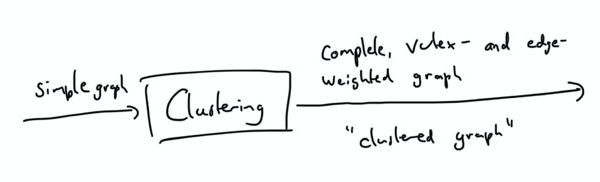
\includegraphics[height=100px]{Resources/Pipeline-Clustering.png}
	\caption{Input and output of the clustering phase.}
	\label{fig:pipeline-clustering}
\end{figure}

Vertices in the cluster graph correspond to clusters in the primal graph and are weighted by the size of the corresponding clusters, \ie{} the number of vertices in the clusters. Edges in the cluster graph represent the similarity of two clusters, \ie{} the number of edges going from one cluster to the other, and are weighted accordingly. Without loss of generality we assume the cluster graph to be complete, meaning that an edge exists between every pair of vertices \emdash{} missing edges can simply be added with a weight of zero.

The cluster graph is the foundation of the map we are going to create: its vertices and their weights are the regions and their desired areas of the map. A subset of its edges will be represented in the map by the border between two countries.

% concrete implementations define what a cluster is -> add this to static part